\chapter{Intégration des applications d'une variable complexe}
\section{Intégration le long d'un chemin}
On rappelle qu'une forme différentielle $\omega$ de degré 1, définie sur un
domaine $U$ de $\mathbb{C}$ et à valeurs dans $\mathbb{C}$, admet une écriture:
\[
\omega=\alpha dz + \beta d\overline{z}
\]
Une telle forme peut s'intégrer le
long d'un chemin de classe $C^1$ par morceaux $\gamma \colon [0,1] \to U$ et, conformément aux résultats du chapitre 8, on a:
\[
\int_{\gamma} \omega = \int_{[0,1]}\left(\alpha \circ \gamma\right)(t)
\gamma^\prime(t)dt + \int_{[0,1]}\left(\beta \circ \gamma\right)(t)
\overline{\gamma^\prime}(t)dt
\]
Soit une application continue $f \colon U \to \mathbb{C}$, on peut lui associer
de façon canonique deux formes différentielles de degré 1, $fdz$ et 
$f d\overline{z}$. On définira:
\[
\int_{\gamma}f dz = \int_{[0,1]}f\left(\gamma(t)\right)\gamma^\prime(t)dt
\]
et 
\[
\int_{\gamma}f d\overline{z} =
\int_{[0,1]}f\left(\gamma(t)\right)\overline{\gamma^\prime}(t)dt
\]

La première expression est appelée intégrale de $f$ le long du chemin $\gamma$.
 Cette formule permet le calcul de nombreuses
intégrales le long de chemins de classe $C^1$. On va par exemple rechercher la
valeur de ~:
\[
\int_{\gamma} \frac{dz}{z}
\]
où $\gamma$ est le chemin $[0, 1] \to \mathbb{C}$ tel que
$\gamma(\theta) = \exp(i 2 \pi \theta)$. L'image de ce chemin est le cercle
unité de $\mathbb{C}$. Il est parcouru une seule fois dans le sens
trigonométrique. On a~: $\gamma^\prime(2 \pi \theta) = i 2 \pi \exp(i 2
\pi \theta)$ et~:
\[
\int_{\gamma} \frac{dz}{z} =  \int_0^1 \exp(-i 2 \pi \theta) (i 2 \pi \exp(i
2 \pi \theta)) d \theta = i 2 \pi 
\]

On peut évaluer l'intégrale de la même application relativement à
$d\overline{z}$:

\begin{align*}
\int_{\gamma} \frac{d\overline{z}}{z} & =  \int_0^1 \exp(-i 2 \pi \theta) (-i 2
\pi \exp(-i 2 \pi \theta)) d \theta  \\
&= -i 2 \pi \int_0^1 \exp(-i4 \pi \theta)
d \theta = 0
\end{align*}



\begin{fprop}
Soit $\gamma : \, [0,1] \to \mathbb{C}$ un chemin de classe $C^1$ par morceaux et soit
$f$ une application  intégrable le long de $\gamma$. Alors~:
\[
\left|\int_{\gamma} f(z) dz\right | \leq \int_{[0,1]} \left |f(\gamma(t)) \right | \left |\gamma^\prime(t) \right | dt
\]
\end{fprop}
On peut obtenir facilement ce résultat en utilisant les sommes de Riemann-Stieltjes.
Cette majoration est utilisée pour obtenir un résultat très utile en
pratique~: le lemme de Jordan.

\begin{fprop}(Lemme de Jordan)\label{prop:jordan}
Soit $\gamma_r$ le chemin formé d'un arc de cercle de rayon $r$, de centre $z_0$ parcouru
 dans le sens trigonométrique, d'angle initial $\alpha_0$ et d'angle final
 $\alpha_1$. Soit $f$ une application continue sur $\gamma_r$ pour
 tout $r>0$. Si la borne supérieure de l'application $|(z-z_0)f(z)|$ tend vers 0 lorsque $r$ 
 tend vers $0$ (resp. $+\infty$), alors~:
\[
\lim_{r \to 0^+ (resp. +\infty)} \int_{\gamma_r} f(z) dz = 0
\]
\end{fprop}
\begin{proof}
Pour $r$ fixé, le chemin $\gamma_r$ s'exprime par:
\[
\gamma_r \colon t \in [0,1] \mapsto z_0 + r e^{i \left(\alpha_0 +
t (\alpha_1 - \alpha_0)\right)}
\]
On a donc:
\[
\left|\int_{\gamma_r} f(z) dz\right| \leq (\alpha_1-\alpha_0) \int_0^1
|f(\gamma_r(t))|r dt 
\]
On remarque par ailleurs que $|(z-z_0)f(z)|=r|f(z)|$ pour $z$ appartenant à
l'image de $\gamma_r$. La conclusion du théorème s'obtient alors directement.
\end{proof}
\section{Formules de Cauchy}
Les résultats de cette section sont fondamentaux pour la suite. Ils vont
permettre en particulier d'établir que tout application holomorphe dans un
domaine y est en fait analytique.
\begin{fdefn}
Un chemin $\gamma \colon [0,1] \to \C$ de classe $C^1$ est dit régulier si $\gamma^\prime(t) \neq 0, \, t \in ]0,1[$. Un chemin de classe $C^1$ par morceaux est régulier s'il l'est sur chaque sous-intervalle où il est continûment différentiable. 
\end{fdefn}
\begin{fthm}(Stokes complexe)\label{thm:stokes_complexe} Soit $\Omega$ un domaine de $\mathbb{C}$
admettant pour bord $\partial \Omega$ un lacet simple régulier de
classe $C^1$ par morceaux. Soit $f : \mathbb{C} \to \mathbb{C}$
application de classe $C^1$ dans $\Omega$ (au sens $\mathbb{R}^2$) et continue
sur $\Omega \cup \partial \Omega$. Alors~:
\[
\int_{\partial \Omega} f(z) dz = - \int_{\Omega} \frac{\partial
f}{\partial \overline{z}} dz d\overline{z}
\]
où l'intégrale en partie droite est faite en considérant $z,\overline{z}$ comme des variables indépendantes.
\end{fthm}

La preuve de ce théorème, qui est essentiellement une application de la formule
de Stokes, va être détaillée à l'aide de deux lemmes fondamentaux.
\begin{lemme}
Soit $\gamma \colon [0,1] \to \mathbb{C}$ un lacet simple régulier de
classe $C^1$. Il existe un nombre fini de couples $(U_i, \theta_i)_{i=1\dots N}$ avec $U_i$
ouvert de $\mathbb{R}^2$ et $\theta_i$ difféomorphisme de classe $C^1$ de $U_i$
dans $\mathbb{R}^2$ vérifiant les assertions suivantes:
\begin{enumerate}
  \item la famille $(U_i)_{i=1\dots N}$ forme un recouvrement ouvert de l'image
  de $\gamma$.
  \item l'image de $\gamma([0,1])\cap U_i$ par $\theta_i$ est un segment de
  l'axe des abscisses.
\end{enumerate}
\end{lemme}
\begin{proof}
Soit $\gamma(t_0)$ un point de l'image de $\gamma$. On a, par régularité de
$\gamma$,  $\gamma^\prime(t_0) \neq 0$. 
Soit l'application:
\[
(t,s) \to \gamma(t) + s v
\]
définie pour $t$ assez proche de $t_0$. Sa dérivée en $(t_0,0)$ a pour matrice
jacobienne:
\[
\left(
\gamma^\prime(t_0), v
\right)
\]
qui est inversible. Le théorème d'inversion locale montre alors qu'il existe un
voisinage ouvert $U_{t_0}$ contenant $\gamma(t_0)$ et un difféomorphisme
$\theta_{t_0}$ de classe $C^1$ défini sur $U$ tel que $\theta_{t_0}(U_{t_0})$
contienne un pavé $]t_0-\epsilon, t_0+\epsilon[ \times ]-\eta, \eta[$ avec
$\epsilon >0, \eta > 0$. Pour tout $t \in ]t_0-\epsilon, t_0+\epsilon[$, on a
$\theta^{-1}(t,0)=\gamma(t)$ par construction. En revanche, il peut exister des
couples $(t,s), s \neq 0$ tels que $\theta^{-1}(t,s)=\gamma(\tilde{t})$, et dans
ce cas $\tilde{t} \notin ]t_0-\epsilon, t_0+\epsilon[$. Soit $\Delta$ l'ensemble
de ces couples. Il existe un pavé $]t_0-\epsilon_1, t_0+\epsilon_1[ \times
]-\eta_1, \eta_1[$ avec $\epsilon_1 > 0$, $\eta_1 > 0$ et ne rencontrant pas
$\Delta$. Supposons cette propriété fausse. Il existe alors une suite de points
$(t_i,s_i)$, $s_i \neq 0$ de limite $(t_0,0)$. Pour tout entier $i$, soit
$\tilde{t}_i$ un point tel que $\gamma(\tilde{t}_i)=\theta^{-1}(t_i,s_i)$. La
suite $\tilde{t}_i, i\in \mathbb{N}$ appartient au compact $[0,1]$ et admet un point
d'accumulation $\tilde{t} \notin ]t_0-\epsilon, t_0+\epsilon[$. Par continuité
de $\gamma$, $\gamma(\tilde{t})=\gamma(t_0)$, ce qui contredit le fait que
$\gamma$ soit un homéomorphisme. On peut donc choisir l'ouvert $U_{t_0}$ de
telle sorte que l'image de $\gamma([0,1]\cap U_{t_0})$ soit un segment de l'axe
des abscisses.
La preuve du lemme se déduit directement de cette propriéte et de la compacité
de $\gamma([0,1])$: La famille $(U_t)$ forme un recouvrement ouvert de
$\gamma([0,1])$, on peut donc en extraire une sous-famille finie qui répond aux
conditions du lemme.
\end{proof}
% Ce lemme permet d'obtenir une forme affaiblie de théorème de Jordan.
%Pour ce faire, on va montrer qu'il existe une partition de $\mathbb{R}^2$ en points
%d'indice nul et points d'indice égal à $\pm 1$ (le signe étant toujours le
%même). On se donne une courbe de Jordan régulière $\gamma$ de classe $C^1$.
%Soit $x \in \mathbb{R}^2$ et soit $v$ un vecteur quelconque non nul. Si la
%demi-droite de sommet $x$ et de vecteur directeur $v$ a une intersection vide
%avec l'image de $\gamma$, l'indice de $x$ est 0: en effet, les points de la
%demi-droite suffisamment loin de l'origine sont d'indice nul et par continuité
%de l'indice, $x$ doit aussi avoir un indice nul. Sinon, il existe un nombre fini
%de domaines $u_i$ dans lesquels une intersection a lieu. En modifiant
%éventuellement $v$, il est toujours possible de supposer que les intersections 
%sont réduites à un point. On raisonne de la façon suivante: en partant d'un
%point de la demi-droite d'indice 0, on chemine vers $x$ (i.e. selon la
%direction $-v$) jusqu'au premier point d'intersection $x_1$. Après
%transformation par le difféomorphisme $\theta_1$ correspondant à l'ouvert $U_1$
%contenant $x_1$, on compare le sens de parcours du chemin et celui du parcours
%de la demi-droite. Si les deux vecteurs sont en sens direct, on augmente d'une
%unité l'indice des points placés après l'intersection, sinon on le diminue d'une
%unité. Cette procédure est schématisée figure \ref{fig:jordan} et s'explique très
%facilement: dans un cas le chemin s'enroule en sens trigonométrique autour des points situés
%après l'intersection, l'indice doit donc augmenter, dans l'autre cas il doit
%diminuer. On répète l'opération de proche en proche jusqu'à atteindre le point
%$x$. Trois cas uniquement peuvent se présenter: l'index de $x$ vaut $0$
% s'il y a eu un nombre pair d'intersections, et $+1$ ou $-1$ s'il y en a eu un
% nombre impair (les signes aux intersections doivent en effet s'alterner, sans
% quoi on ne pourrait avoir un lacet simple). Pour la même raison, il n'est pas
% possible d'avoir à la fois des points d'indice $+1$ et $-1$. L'ensemble des
% points d'indice non nul forme un domaine de $\mathbb{R}^2$, de bord l'image de
% $\gamma$ et ceux d'indice nul un domaine non borné, ce qui est précisément la
% conclusion du théorème de Jordan.
% \begin{figure}[ht]
%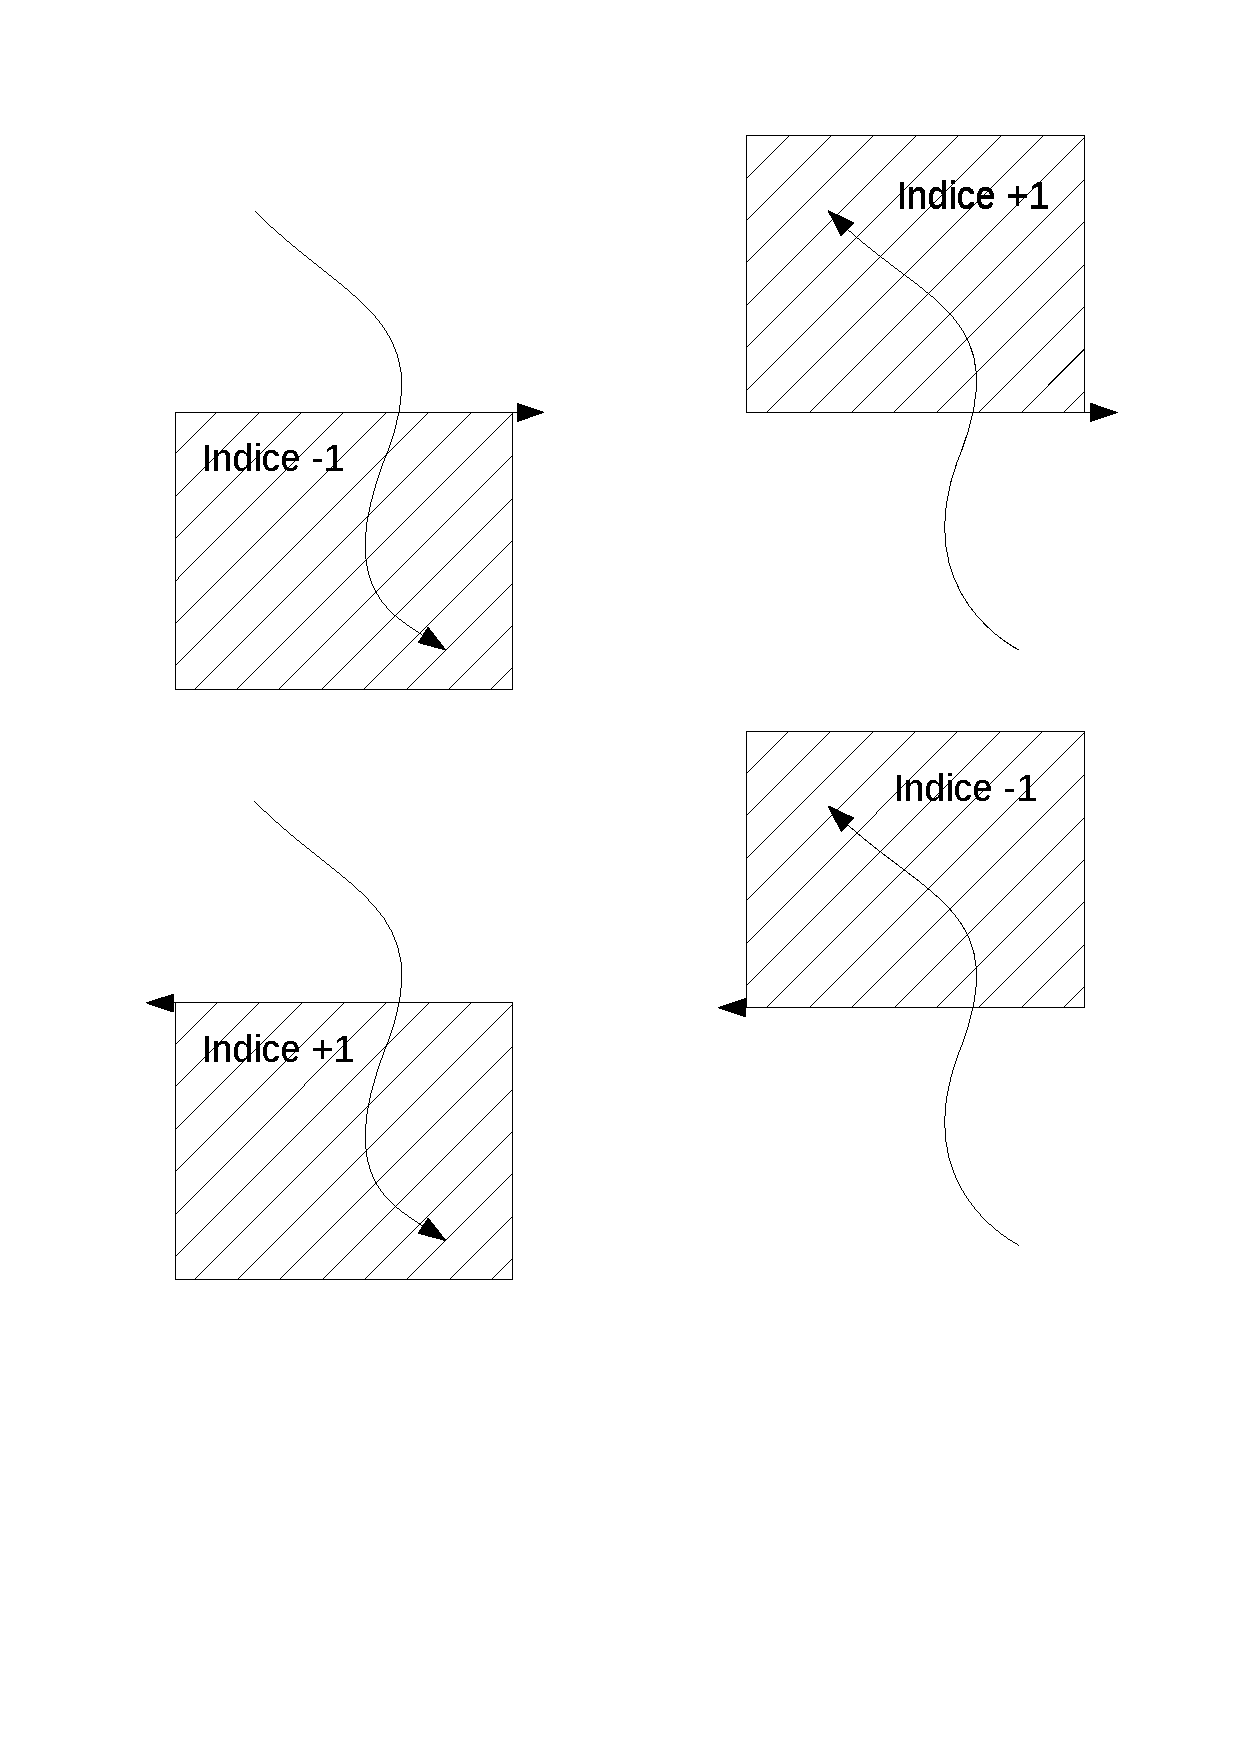
\includegraphics[scale=0.3]{images/jordan.pdf}
%\caption{Franchissement d'un lacet}\label{fig:jordan}
%\end{figure}
%On peut utiliser de façon pratique le procédé précédent pour déterminer
%rapidement si un point appartient au domaine intérieur à une courbe de Jordan;
%c'est un algorithme que l'on rencontre couramment dans les logiciels de dessin
%ou de conception assistée par ordinateur, en concurrence avec celui basé sur un
%calcul de l'indice par intégration que nous verrons plus loin.
%
%On notera la latitude laissée dans le choix de la direction $v$ utilisée dans
%la preuve du lemme. En particulier, si $U$ est le domaine intérieur à $\gamma$,
%on pourra toujours choisir les difféomorphismes $\theta_i$ de telle façon 
%que l'image de  $U \cap U_i$ par $\theta_i^{-1}$ soit contenue dans le
%demi-espace $\mathbb{R}\times \mathbb{R}^+$. La portion de courbe $\gamma$,
%forme un segment de l'axe des abscisses et sera parcouru soit dans le sens des 
%abscisses croissantes, soit dans le sens des abscisses décroissantes. 
%Dans le premier cas, l'indice devra être +1 pour les points intérieurs
%et donc -1 dans le second cas. 
%L'indice étant constant, on en déduit que le sens de parcours sera le même dans
%tous les morceaux obtenus par applications des $\theta_i^{-1}$. On dira que $\gamma$ est
%orientée en sens positif si l'indice des points intérieurs est +1, en sens
%négatif s'il vaut -1. L'orientation d'une courbe de Jordan est toujours
%possible, mais ceci ne reste plus vrai en dimension supérieure, même pour des
%surfaces très régulières: des exemples de surfaces $C^\infty$ non orientables
%peuvent facilement être obtenus.

Le lemme peut être étendu à un chemin de classe $C^1$ par morceaux:
\begin{lemme}
Soit $\gamma$ un lacet simple régulier de classe $C^1$ par morceaux. Il
existe pour tout point $t_0$ où la dérivée de $\gamma$ est discontinue un voisinage ouvert
$U$ de $\gamma(t_0)$ dans $\mathbb{C}$,un voisinage ouvert $V$ de $(t_0,0)$ dans
$\mathbb{R}^2$ et un difféomorphisme $\theta$ de classe $C^1$ de $U$ dans $V$
tels que l'image de $\gamma([0,1]) \cap U$ soit la réunion d'un segment du
demi-axe des abscisses négatif et d'un segment de l'axe du demi-axe des
ordonnées positif.
\end{lemme}
\begin{proof}
La démonstration est semblable à celle du lemme précédent. On notera $\gamma^-$
(resp. $\gamma^+$) la portion de l'image du lacet $\gamma$ formée des points
$\gamma(t), t < t_0$ (resp. $\gamma(t),t > t_0$). On peut compléter $\gamma^+,
\gamma^-$ dans un voisinage de $t_0$ de telle façon que le chemin ainsi obtenu
soit de classe $C^1$:on peut par exemple prolonger par un segment de droite de
vecteur directeur la limite à gauche (resp. à droite) de la dérivée de $\gamma$
en $t_0$. On continuera à désigner $\gamma^+, \gamma^-$ les chemins ainsi
prolongés. Dans un voisinage de $(t_0,t_0)$, on définit l'application:
\[
(t,s) \mapsto \gamma(t) + \gamma(s) - \gamma(t_0)
\]
Sa matrice Jacobienne en $(t_0,t_0)$ est:
\[
\left(
\gamma^\prime(t_0^-), \gamma^\prime(t_0^+) 
\right )
\]
qui est de rang maximal si $t_0$ est un point de discontinuité de la dérivée. 
Le théorème d'inversion locale permet alors de conclure.
\end{proof}
 Il est maintenant possible de procéder à la preuve du
théorème.
\begin{proof}
On posera $f = P + i Q$. Soit $U$ le domaine intérieur bordé par le lacet simple régulier $\partial \Omega$. Soient enfin $U_i, i=1\dots N$ les ouverts
donnés par le premier ou le second lemme selon que l'on est ou non au voisinage
d'un point de discontinuité de la dérivée. Le recouvrement ouvert $U \cup
\bigcup_{i=1}^N U_i$ admet une partition de l'unité $\alpha_i, i=0\dots N$ subordonnée 
(on note $\alpha_0$ le terme associé à $U$). Considérons les formes différentielles continues de
degré 1:
\[
\omega_1 = P dx - Q dy, \quad \omega_2= Qdx + Pdy 
\]
on a:
\[
d\omega_1 = -\left(\frac{\partial P}{\partial y}+\frac{\partial Q}{\partial
x}\right )dx \wedge dy
\]
et
\[
d\omega_2 = \left(\frac{\partial P}{\partial x}-\frac{\partial Q}{\partial
y}\right )dx \wedge dy
\]
L'intégrale:
\[
\int_{U} \alpha_0 d\omega_1 = - \int_{U}\alpha_0(x,y) \left(\frac{\partial
P}{\partial y}(x,y)+\frac{\partial Q}{\partial x}(x,y)\right )dxdy
\]
vaut $0$, le support de $\alpha_0$ se trouvant dans $U$. La même propriété
est vraie pour $d\omega_2$. Soit maintenant un des ouverts $U_i, i=1\dots N$ et
$\theta_i^{-1}$ le difféomorphisme de classe $C^1$ associé (on choisit de
travailler avec $\theta_i^{-1}$ pour simplifier les notations). On remarquera
tout d'abord (le vérifier !) que $\theta_i^*\left(\alpha_i d \omega_1\right) =
\alpha_i\circ \theta_i d \theta_i^* \omega_1$. On a donc:
\[
\int_{U_i} \alpha_i d \omega_1  = \int_{\theta_i(U_i)} \alpha_i\circ \theta_i d
\theta_i^* \omega_1
\]
La formule de Stokes élémentaire (qui s’étend très facilement dans le
cas des images d'ouverts contenant une singularité) appliquée à l'ouvert
$\theta_i(U_i)$ montre que l'intégrale précédente vaut $\int_{\theta_i(\gamma[0,1]\cap U_i)} 
\left (\alpha_i \circ \theta_i\right) \theta_i^*(\omega_i)$ qui s'identifie à
l'intégrale de la partie réelle de $f$ sur la portion de chemin appartenant à
$U_i$. Un raisonnement similaire peut se faire sur $\omega_2$: on en déduit le
théorème par sommation sur les $U_i$.
\end{proof}
Ce théorème permet d'obtenir un corollaire très simple, mais très utile: si $f$
vérifie les hypothèses précédente et est holomorphe, alors l'intégrale le long
de $\partial \Omega$ vaut 0. 
La formule \ref{thm:stokes_complexe} n'est pas valable pour des domaines présentant des trous, tels celui de la figure \ref{fig:domaine_trois_connexe}.
\begin{figure}[ht]
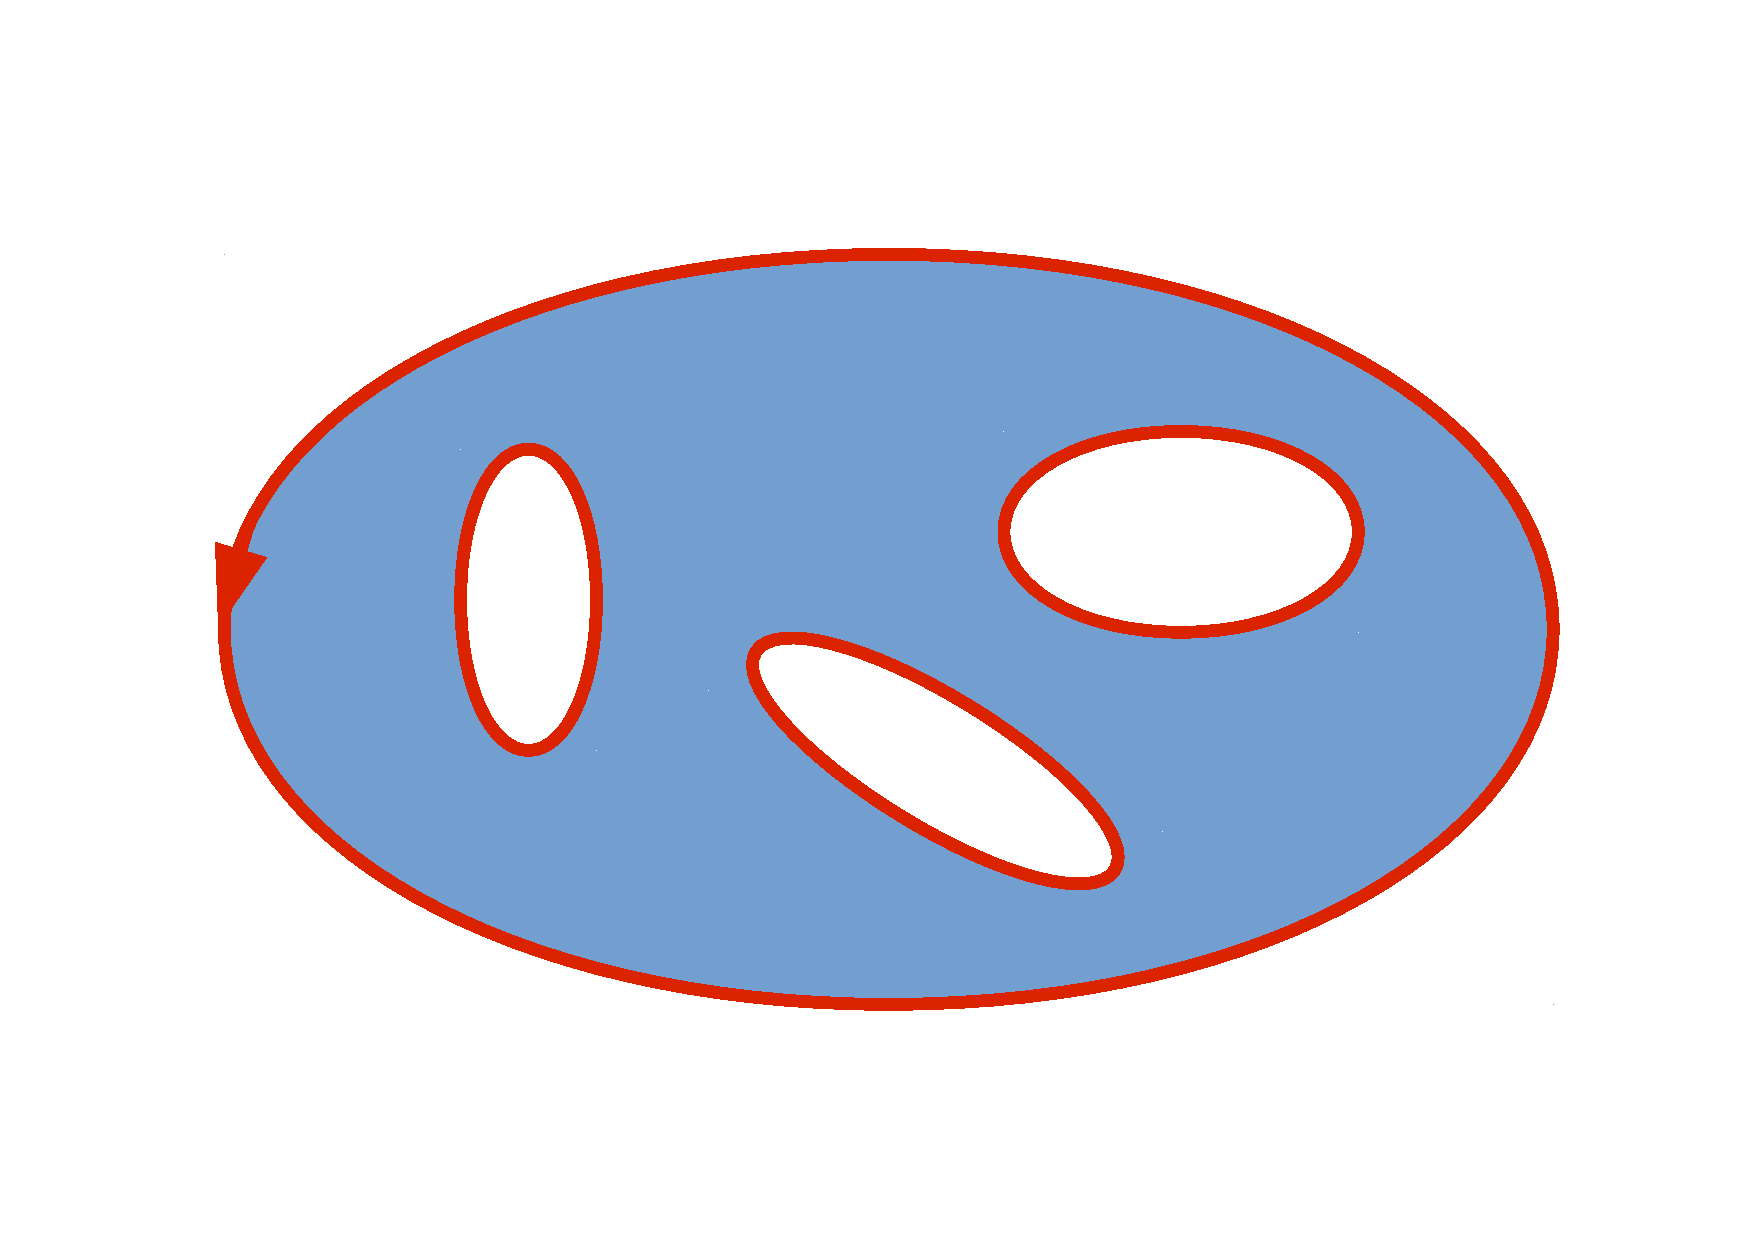
\includegraphics[scale=0.3]{images/domaine_trois_connexe.pdf}
\caption{Domaine 3-connexe}\label{fig:domaine_trois_connexe}
\end{figure}
Si le bord est formé d'une union disjointe de lacets simples réguliers de classe $C^1$, on peut néanmoins continuer à appliquer le théorème en prenant garde à orienter en sens direct le contour extérieur et en sens rétrograde les lacets internes. 

Le théorème qui vient d'être énoncé permet de calculer des intégrales de la
variable réelle difficiles à obtenir de façon directe. L'exercice suivant permet 
d'évaluer les intégrales de Fresnel, que l'on rencontre assez fréquemment en
physique (ces intégrales sont issues d'un problème d'optique).
\begin{exercice}
Soit l'application $f \colon z \mapsto \exp\left(i z^2\right)$. 
\begin{itemize}
  \item Montrer que $f$ est holomorphe sur $\mathbb{C}$ et vérifier que sa
  dérivée est continue.
  \item Pour tout réel $r > 0$, le contour $\gamma_r$ est défini selon la figure
  \ref{fig:contour2}. Donner la valeur de l'intégrale:
  \[
  \int_{\gamma_r} f(z) dz
  \]
  \item Écrire cette intégrale sous la forme d'une somme de trois
  intégrales de chemin et montrer que l'intégrale correspondant à l'arc de
  cercle tend vers 0 lorsque $r \to +\infty$.
  \item En déduire les valeurs des intégrales généralisées suivantes, dites
  intégrales de Fresnel:
  \[
  \lim_{r \to +\infty} \int_{[-r,r]} \cos(x^2) dx, \quad  \lim_{r \to +\infty}
  \int_{[-r,r]} \sin(x^2) dx
  \]
\end{itemize}
\end{exercice}
 \begin{figure}[ht]
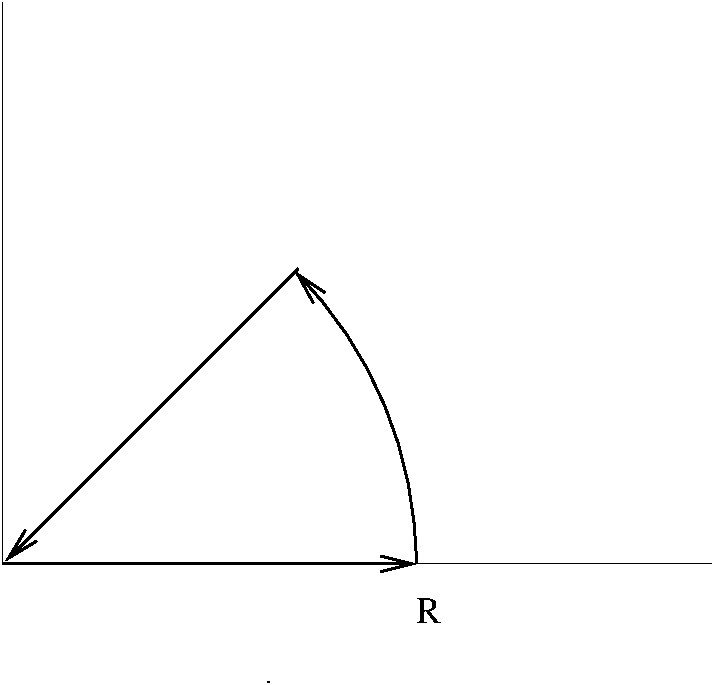
\includegraphics[scale=0.3]{images/contour_fresnel.pdf}
\caption{Contour $\gamma_r$}\label{fig:contour2}
\end{figure}
On utilise fréquemment les techniques d'intégration dans le plan complexe pour
obtenir des transformées de Fourier. L'exercice suivant calcule la transformée
de Fourier d'une gaussienne, qui a déjà été obtenue précédemment à l'aide d'une
équation différentielle. 
\begin{exercice}
Soit $f \colon z \in \mathbb{C} \mapsto \exp(-z^2)$.
\begin{itemize}
  \item Montrer que $f$ est holomorphe dans $\mathbb{C}$, de dérivée continue.
  \item En utilisant le contour $\gamma_r$ donné figure , déterminer, pour
  $\omega \in \mathbb{R}$ fixé, la valeur de l'intégrale:
  \[
  \int_{\gamma_r} \exp(-z^2)dz
  \]
  \item En faisant tendre $r$ vers $+\infty$ et en faisant un raisonnement
  similaire à celui de l'exercice précédent, déterminer la transformée de
  Fourier de l'application $x \mapsto \exp(-x^2)$.
\end{itemize}
\end{exercice}
 \begin{figure}[ht]
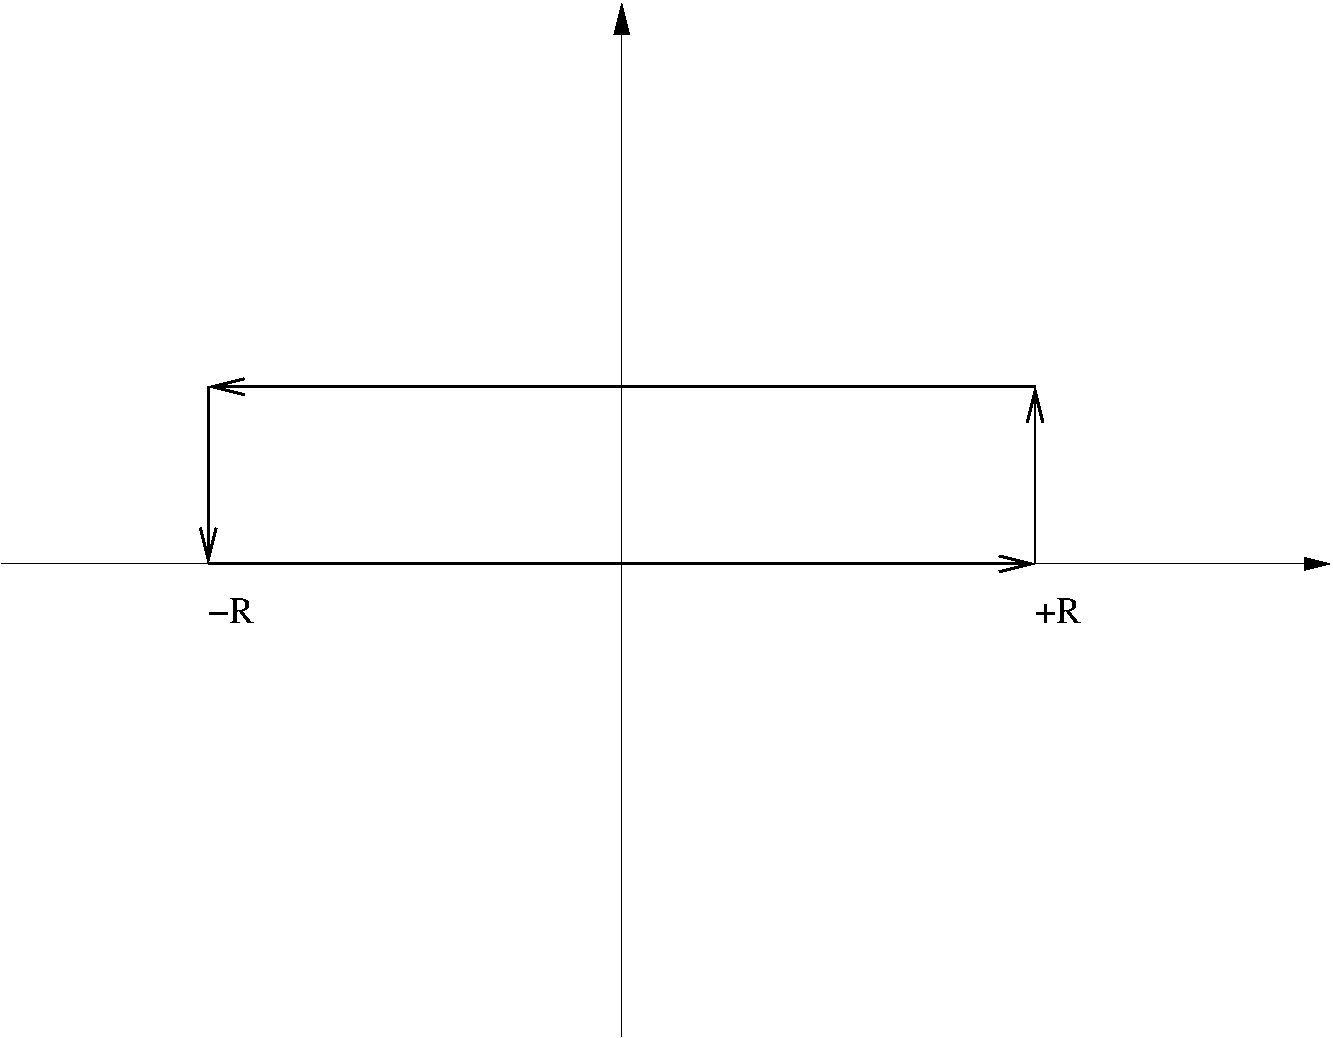
\includegraphics[scale=0.3]{images/contour_gauss.pdf}
\caption{Contour $\gamma_r$}\label{fig:contour3}
\end{figure}

La formule \ref{thm:stokes_complexe} montre qu'une application holomorphe et de dérivée continue dans un domaine (éventuellement avec des trous) a une intégrale nulle le long du bord. Nous allons maintenant montrer que cette propriété subsiste sous des hypothèses plus larges. 
\begin{fdefn}
Un lacet triangulaire de sommets $z_0,z_1,z_2$ est un lacet simple régulier de
classe $C^1$ par morceaux qui constitue le bord d'un triangle du plan complexe
de sommets $z_0,z_1,z_2$.
\end{fdefn}

Ce type de chemins joue un rôle particulier en théorie de l'intégration. La
propriété suivante est simple, mais fondamentale.

\begin{fprop}(Existence d'une primitive locale)
Soit $\Omega$ un domaine de $\mathbb{C}$ et $f \colon \Omega \to \mathbb{C}$ une
application continue. Si l'intégrale de $f$ le long de tout lacet triangulaire
de $\Omega$ est nulle, alors au voisinage de tout point $z_0 \in \Omega$, il
existe une application holomorphe $F$ de dérivée égale à $f$.
\end{fprop}

\begin{proof}
Soit $z_0 \in \Omega$ et soit $B_{z_0}$ une boule ouverte centrée en $z_0$ et
contenue dans $\Omega$. On pose, pour tout $z \in
B_{z_0}$:
\[
F(z) = \int_0^1 f(z_0 + t(z-z_0))(z-z_0) dt
\]
Soit maintenant $z \in B_{z_0}$ et soit $h \in \mathbb{C}$ tel que
$z+h \in B_{z_0}$. On a, en considérant le lacet triangulaire figure
\ref{fig:morera}:
\begin{align*}
F(z+h)-F(z) &= \int_0^1 f(z_0 + t(z-z_0))(z-z_0) dt \\
& - \int_0^1 f(z_0 +
(1-t)(z + h -z_0))(z + h-z_0) dt \\
&= \int_0^1 f(z+th)h dt 
\end{align*}
Par continuité de $f$, on en déduit:
\[
\lim_{h \to 0} \frac{F(z+h)-F(z)}{h} = f(z)
\]
ce qui prouve que $F$ est holomorphe, de dérivée $f$ en tout point de
$B_{z_0}$. 
\end{proof}
 \begin{figure}[ht]
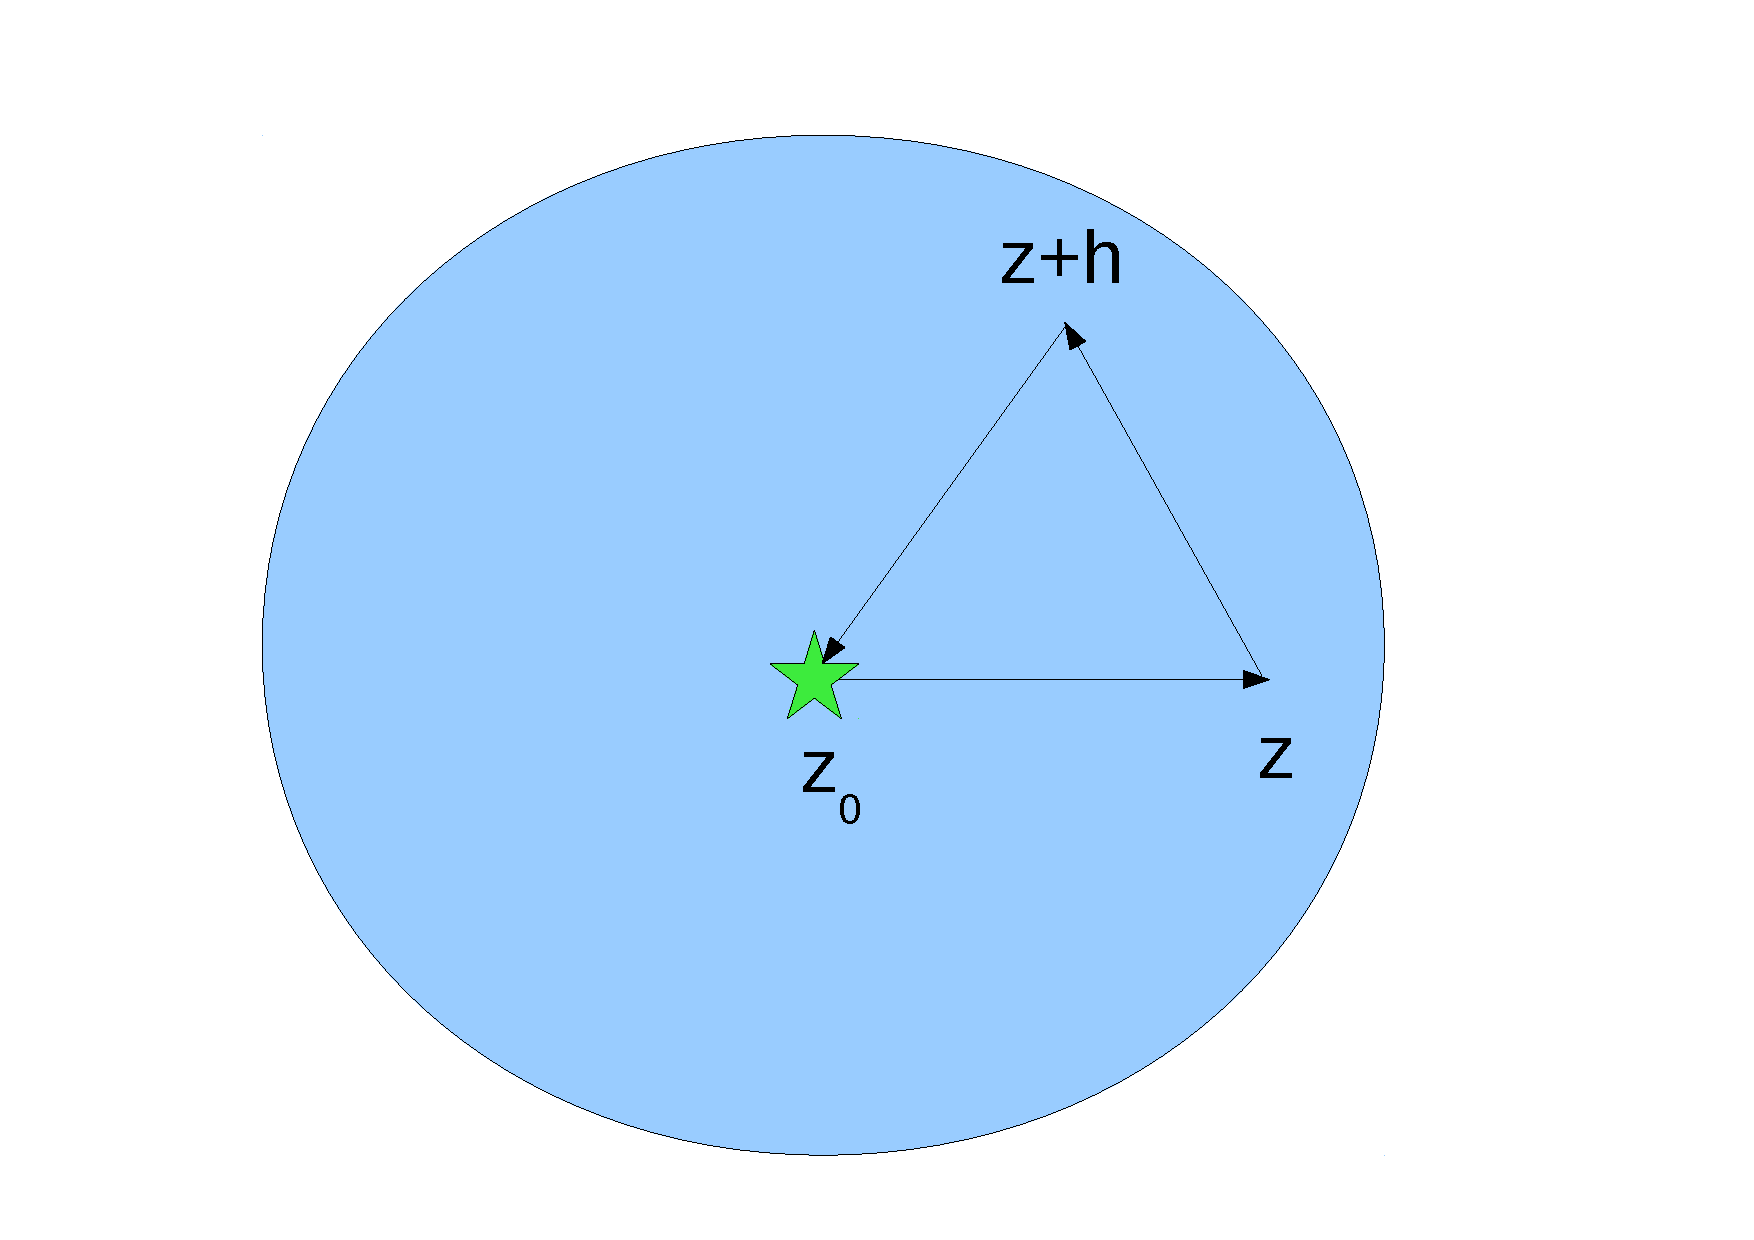
\includegraphics[scale=0.3]{images/morera.pdf}
\caption{Lacet triangulaire}\label{fig:morera}
\end{figure}
On notera que si $F$ est une primitive locale, il en est de même pour $F+K$ où
$K$ est un complexe quelconque.

\begin{fprop}(Primitive le long d'un chemin)
Soit $\Omega$ un domaine de $\mathbb{C}$ et soit $f$ vérifiant les hypothèses
de la proposition précédente. Soit $\gamma$ un chemin de $\Omega$. Il existe
alors une application continue $\theta \colon [0,1] \to \mathbb{C}$ telle 
que pour tout $t \in [0,1]$, il existe un voisinage $V_t$ de $\gamma(t)$
dans $\Omega$, une application $F$, holomorphe de classe $C^1$ sur $V_t$, de
dérivée égale à $f$ et vérifiant $\theta(u)=F(\gamma(u))$ au voisinage de $t$.
\end{fprop}

\begin{proof}
On va montrer par un procédé constructif la possibilité d'obtenir $\theta$. On
choisit tout d'abord $\theta_0$ de façon arbitraire. L'image de $\gamma$ est
un compact, on peut donc la recouvrir par un nombre fini de boules ouvertes
$B_i, i=1\dots N$ sur lesquelles on peut obtenir (proposition
précédente) une application $F_i$ holomorphe de classe $C^1$ et telle que
$F_i^\prime = f$. De plus, quitte à réordonner la numérotation des boules $B_i$,
on peut obtenir une subdivision $0=t_0 < t_2 < \dots < t_N = 1$ de $[0,1]$
telle que $\gamma([t_{i-1},t_i])\subset B_i, i =1\dots N$. 
 On peut choisir $F_1$ de telle sorte que
$F_1(\gamma(0))=\theta_0$ et on pose pour $u \in [t_0,t_1]$,
$\theta(u)=F_1(\gamma(u))$.
Supposons obtenue $\theta$ jusqu'à $t_i$. Sur le domaine $B_i \cap B_{i+1}$, la
différence entre $F_i,F_{i+1}$ est de dérivée nulle, donc cette différence est
constante. On peut choisir $F_{i+1}$ de telle sorte qu'elle soit nulle, ce qui
définit $\theta$ de proche en proche.
\end{proof}
Dans le cas où une application vérifie les hypothèses de la proposition
précédente, on peut définir de façon simple une notion d'intégrale le long du
chemin $\gamma$. Si $\theta$ est une primitive de $f$ le long de $\gamma$, on
posera:
\[
\int_{\gamma} f(z) dz = \theta(1)-\theta(0)
\] 
Cette définition coïncide avec celle donnée précédemment pour les chemins
de classe $C^1$ par morceaux, mais ne fait aucune autre hypothèse que la continuité sur
$\gamma$. En revanche, $f$ doit être continue et vérifier la condition
d'annulation de l'intégrale sur les lacets triangulaires.
L'intégrale est en général dépendante du chemin suivi. On a néanmoins une
invariance par homotopie, très importante pour la suite.
\begin{fdefn}
Soit $\Omega$ un domaine de $\mathbb{C}$ et  $\gamma_1, \gamma_2$ deux
chemins de $\Omega$ tels que $\gamma_1(0) = \gamma_2(0)$ et $\gamma_1(1) = \gamma_2(1)$. On dira que $\gamma_1$ et $\gamma_2$ sont homotopes à extrémités fixées si il existe une application continue:
\[
H \colon [0,1] \times [0,1] \to \Omega
\] 
telle que:
\begin{itemize}
\item $\forall t \in [0,1], \, H(0,t) = \gamma_1(t), \, H(1,t) = \gamma_2(t)$
\item $\forall s \in [0,1], \, H(s,0) = \gamma_1(0) = \gamma_2(0), \, H(s,1) = \gamma_1(1) = \gamma_2(1)$
\end{itemize}
\end{fdefn}
\begin{fthm}(Invariance par homotopie)
Soit $\Omega$ un domaine de $\mathbb{C}$ et soient $\gamma_1, \gamma_2$ deux
chemins de $\Omega$, homotopes à extrémités fixées. Soit $f \colon
\Omega \to \mathbb{C}$ continue et dont l'intégrale le long de tout lacet
triangulaire de $\Omega$ s'annule. Alors:
\[
\int_{\gamma_1} f(z) dz = \int_{\gamma_2} f(z) dz
 \]
\end{fthm}

\begin{proof}
 Soit $H$ l'homotopie entre $\gamma_1$ et $\gamma_2$. Pour tout
point $H(t,s)$, il existe une boule ouverte $B$ centrée sur ce point et contenue
dans $\Omega$ qui est ouvert. Par continuité de $H$, on en déduit l'existence
d'un pavé $]t_1,t_2[\times ]s_1,s_2[$ contenant $(t,s)$ et dont l'image est dans
$B$. La collection de ces pavés forme un recouvrement du compact
$[0,1]\times[0,1]$, il en existe donc une famille finie $\mathcal{S}$ qui
constitue aussi un recouvrement. Comme $\mathcal{S}$ est finie, on peut
construire une subdivision de $[0,1]\times[0,1]$ sous la forme de pavés
$\Delta_{ij}=[t_i, t_{i+1}]\times [s_j,s_{j+1}], \, i=0\dots N-1, j=0,\dots M-1$
avec $t_0=s_0=0$, $t_N=s_M=1$ tels que pour tout couple $(i,j)$,
$H(\Delta_{ij})$ est inclus dans un des membres de la famille $\mathcal{S}$. 
L'intégrale de $f$ étant nulle le long de tout lacet triangulaire, elle admet
une primitive dans chacune des boules de la famille $\mathcal{S}$ (reprendre la
démonstration précédente) et donc l'intégrale de $f$ le long du bord de
$\Delta_{ij}$ est nulle (différence de la primitive en deux points identiques).
De proche en proche, on en déduit que l'intégrale de $f$ le long des chemins $s \mapsto
H(t_i,s)$ est constante, soit finalement que l'intégrale de $f$ le long de
$\gamma_1$ est égale à celle le long de $\gamma_2$.
\end{proof}
L'invariance par homotopie montre en particulier que l'intégrale de $f$ le long
d'un lacet homotope à un lacet constant vaut $0$.

\begin{fdefn}
Soit $\Omega$ un domaine de $\mathbb{C}$. On appelle triangle de $\Omega$ de
sommets $z_1,z_2,z_3$ une partie $T \subset \Omega$ formée des combinaisons
barycentriques $\alpha_1 z_1 + \alpha_2 z_2 + \alpha_3 z_3$ où les
$\alpha_1,\alpha_2,\alpha_3$ appartiennent à $[0,1]$ et
$\alpha_1+\alpha_2+\alpha_3=1$.
\end{fdefn}

Le bord d'un triangle est un lacet triangulaire.

\begin{fthm}(Goursat)
Soit $\Omega$ un domaine de $\mathbb{C}$ et soit $f$ une application holomorphe
dans $\Omega$. Alors pour tout triangle $T$ de $\Omega$, l'intégrale de 
$f$ sur le bord de $T$ est nulle.
\end{fthm}

\begin{proof}
Le théorème de Goursat utilise un argument de division. Soit $T_0$ un 
triangle de $\Omega$ et soit $T_n$ une suite de fermés obtenus par
subdivision de $T_0$, ainsi que mentionné figure \ref{fig:sub_triang}. En posant
$d$ le diamètre de $T_0$ et $p$ son périmètre, on vérifie facilement que le
diamètre des triangles de $T_n$ est $d 2^{-n}$ et que le périmètre est $p
2^{-n}$. Soit $\epsilon > 0$. Il existe, pour tout $z$ intérieur à $T_0$, une
boule ouverte $B_z$ telle que:
\[
\forall u \in B_z, |f(u)-f(z)-f^\prime(z)(u-z)| < \epsilon |u-z|
\]
$T_0$ étant compact, un nombre fini de boules $B_z$ le recouvre. Il existe donc
une subdivision $T_n$ telle que chaque triangle la constituant soit dans l'une
de ces boules. L'application  $u \mapsto f(z)+f^\prime(z)(u-z)$ est un polynôme,
donc holomorphe et de dérivée continue: son intégrale sera nulle sur le
bord chaque triangle de $T_n$. Soit $T$ un triangle de $T_n$ contenu dans la boule $B_z$. 
On a:
\begin{align*}
& \left|
\int_{\partial T} f(u) du
\right| \leq  \\ &\int_{\partial T}  |f(u)-f(z)-f^\prime(z)(u-z)| du + \left |
\int_{\partial T} f(z)+f^\prime(z)(u-z) \right| du \leq \\
& \int_{\partial T}  |f(u)-f(z)-f^\prime(z)(u-z)| du \leq \\
& \epsilon d p 4^{-n}
\end{align*}
$T_n$ étant formé d'exactement $4^n$ triangles, on a par sommation:
\[
\left| \int_{\partial T_0} f(u) du \right| < \epsilon d p
\]
Comme $\epsilon$ est arbitraire, on en déduit que l'intégrale est nulle.
\end{proof}
 \begin{figure}[ht]
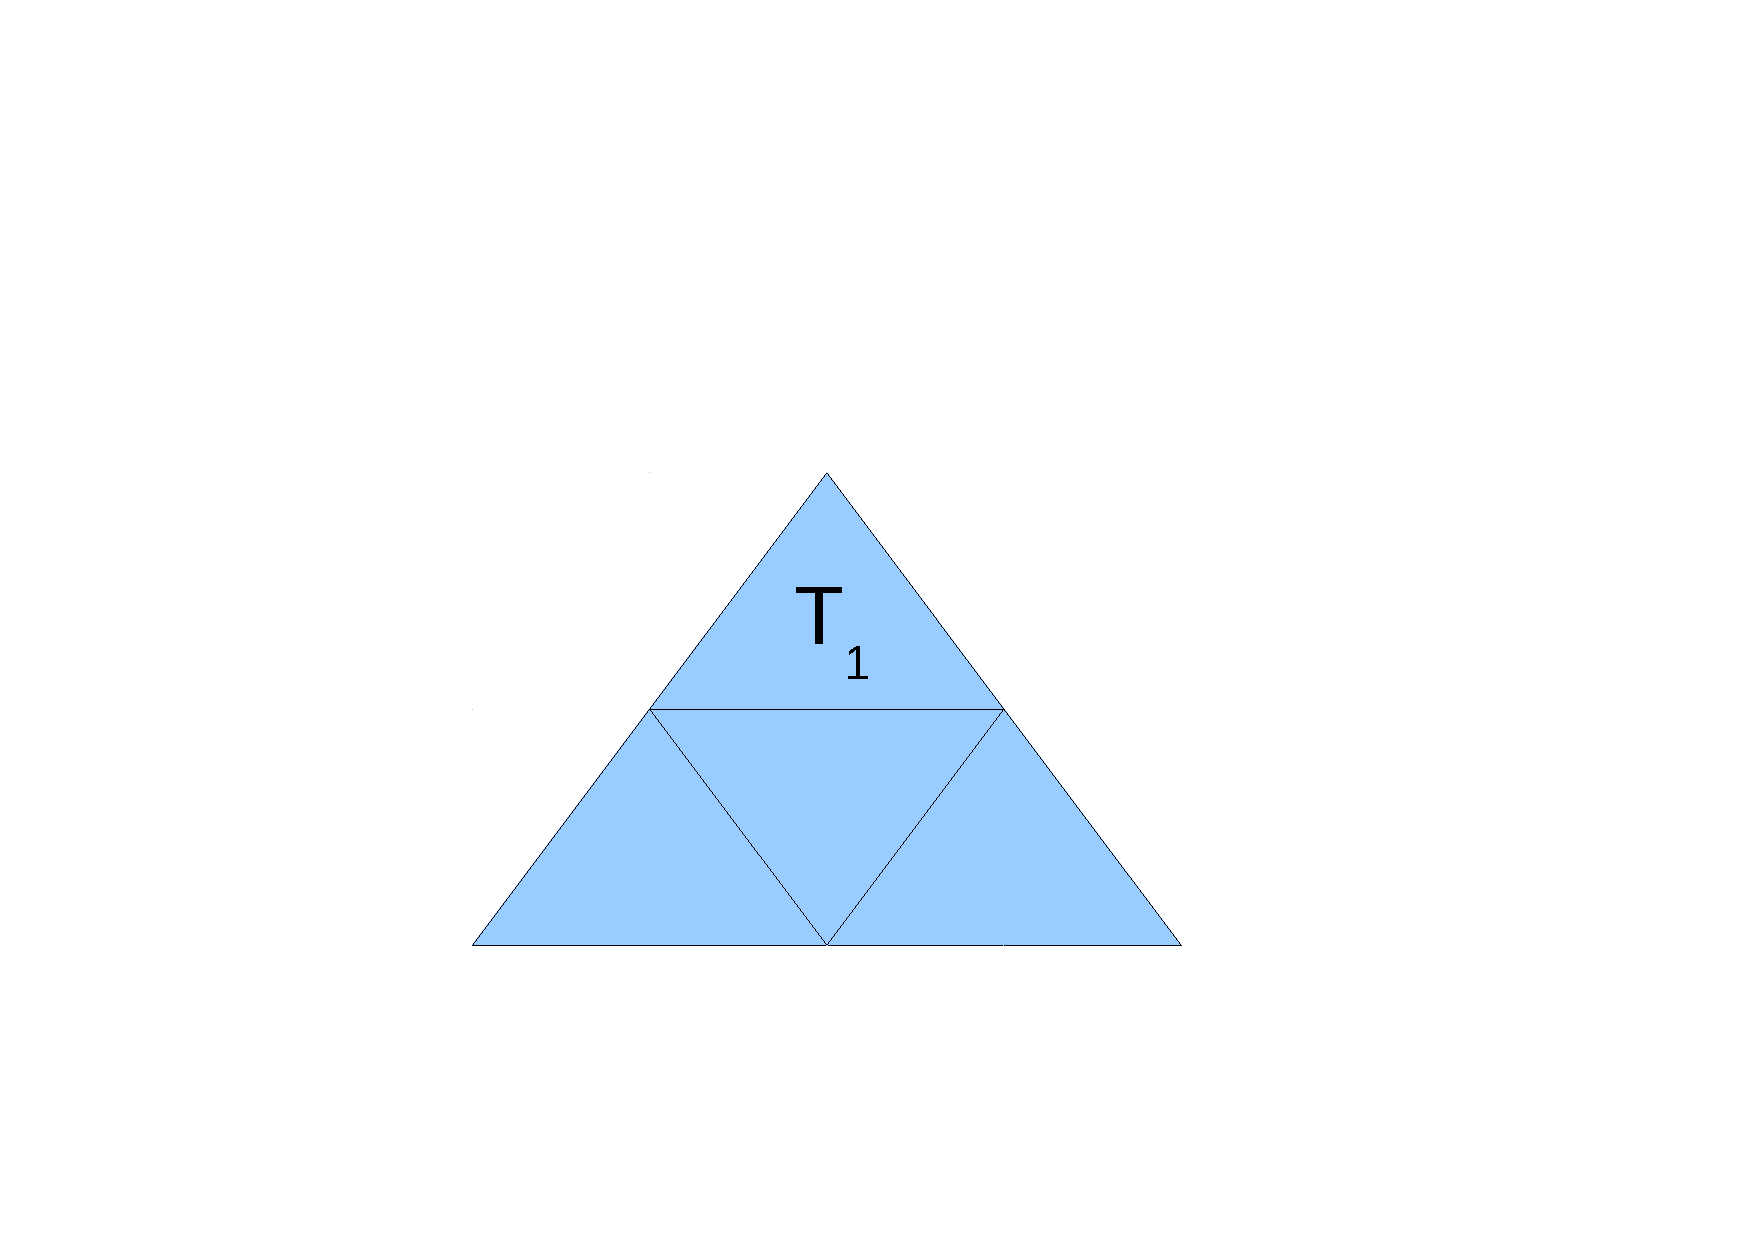
\includegraphics[scale=0.3]{images/subdivision_triangle.pdf}
\caption{Passage de $T_0$ à $T_1$ par subdivision}\label{fig:sub_triang}
\end{figure}
Le théorème de Goursat est encore vrai si l'on suppose seulement l'holomorphie
sur $\Omega$ privé d'une droite et la continuité sur $\Omega$: si la droite en
question coupe un chemin triangulaire on se ramènera par continuité et
subdivision au cas précédent. Dans un domaine $1$-connexe, on a le très important théorème suivant:

\begin{fthm}
Soit $\Omega$ un domaine simplement connexe. Soit $f$ une application holomorphe
dans $\mathbb{C}$. Alors $f$ admet une primitive le long de tout chemin de
$\Omega$ et l'intégrale de $f$ sur tout lacet de $\Omega$ est nulle.
\end{fthm}

\begin{proof}
Le théorème de Goursat montre l'existence d'une primitive pour $f$ le long de
tout chemin de $\Omega$. Le domaine étant simplement connexe, tout lacet est
homotope à un lacet constant: l'intégrale de $f$ le long de tout lacet est
nulle.
 \end{proof}
 Le théorème précédent donne aussi une primitive globale $F$ pour $f$: il
 suffit à cet effet de se donner la valeur de $F$ en un point $z_0 \in \Omega$
 et de poser:
 \[
 F(z) = F(z_0) + \int_{\gamma} f(z)dz
 \]
 avec $\gamma$ chemin d'origine $z_0$ et d'extrémité $z$. L'intégrale de $f$
 est nulle sur tout lacet, la valeur de $F$ en $z$ ne dépend donc pas du chemin
 choisi.
\section{Formules de Cauchy}

\begin{fdefn}(Calcul de l'indice par intégrale curviligne)
Soit $\gamma$ un lacet et  soit $z_0 \in \mathbb{C}$ n'appartenant pas à l'image
de $\gamma$. L'indice de $\gamma$ par rapport à $z_0$ est:
\[
I(\gamma;z_0) = \frac{1}{i 2 \pi}\int_{\gamma} \frac{1}{z-z_0}dz
\]
\end{fdefn}
L'indice d'un lacet compte le nombre de tours effectués par $\gamma$ autour de $z_0$, positivement dans le sens trigonométrique et négativement en sens opposé. On peut établir cette propriété en raisonnant en deux temps. Sans perte de généralité, on supposera que $z_0 = 0$. On note tout d'abord que si $\gamma$ ne passe pas par 0, il existe une boule fermée $B(0,r)$ ne rencontrant pas $\gamma$. L'application:
\[
H \colon (s,t) \in [0,1] \times [0,1] \mapsto s \frac{r \gamma(t)}{|\gamma(t)|} + (1-s) \gamma(t)
\] 
établit une homotopie dans $C^*$ entre $\gamma$ et un lacet $\tilde{\gamma} = H(1,\bullet)$ dont l'image appartient au cercle $\mathcal{C}_r$ de centre 0 et de rayon $r$. En vertu du théorème d'invariance homotopique, l'indice de $\tilde{\gamma}$ est le même que celui de $\gamma$. Au voisinage de $\mathcal{C}_r$, l'application:
\[
\ln \left(z = |z|\exp(i \theta) \right) = \ln |z| + i (\theta+ 2 k \pi), \theta \in [0, 2 \pi [ , k \in \Z
\]
définit une primitive locale de l'application $z^{-1}$ et la conclusion s'ensuit (faire un dessin et propager les écarts angulaires \dots). 
\begin{fthm}(Première formule de Cauchy)
Soit $\Omega$ un domaine simplement connexe de $\mathbb{C}$ et $f$ holomorphe
dans $\Omega$. Soit $\gamma$ un lacet de $\Omega$ et $z_0$ n'appartenant pas à
l'image de $\gamma$. On a:
\[
\int_{\gamma} \frac{f(z)}{z-z_0} dz = i 2 \pi I(\gamma; z_0)f(z_0)
\]
\end{fthm}
\begin{proof}
Soit l'application:
\[
F \colon z \mapsto \left \{
\begin{array}{cc} 
\frac{f(z)-f(z_0)}{z-z_0} & z \neq z_0 \\
f^\prime(z_0) & z = z_0
\end{array}
\right.
\]
$F$ est holomorphe dans $\Omega - \{z_0\}$, continue sur $\Omega$: le théorème
de Goursat (forme étendue) montre que l'intégrale de $F$ le long de $\gamma$ est
nulle, la conclusion est obtenue avec la proposition établie sur le calcul de
l'indice par intégrale curviligne.
\end{proof}
La formule de Cauchy peut également s'énoncer dans le cas d'un domaine dont le
bord est un lacet simple régulier de classe $C^1$ par morceaux:

\begin{fprop}
Soit $\Omega$ un domaine de bord $\partial \Omega$ un lacet simple régulier de classe $C^1$ et soit $f$ une application holomorphe dans $\Omega$,
continue sur $\partial \Omega$. Pour tout point $z_0 \in \Omega$ on a:
\[
\int_{\gamma} \frac{f(z)}{z-z_0} dz = i 2 \pi f(z_0)
\]
\end{fprop}
 
La preuve est similaire au cas précédent, mais utilise le théorème basé sur la
formule de Stokes.
 La formule de Cauchy se généralise immédiatement au cas d'un domaine
 $n$-connexe dont le bord est constitué d'une union finie de lacets simples rectifiables, en se ramenant à un ouvert simplement connexe. On prendra
garde néanmoins au sens de parcours du lacet.

 \begin{fthm}(Seconde formule
de Cauchy) Sous les même hypothèses que la première formule de Cauchy, on a~:
\[
I(\gamma; z_0) f^\prime(z_0) = \frac{1}{i 2 \pi} \int_{\gamma}
\frac{f(z)}{(z-z_0)^2} dz
\]
\end{fthm}

\begin{proof}
On supposera l'indice du lacet $\gamma$ égal à 1 pour simplifier les écritures.
Formons le rapport~:
\[
\frac{f(z_0+h)-f(z_0)}{h} = \frac{1}{i 2
\pi}\int_{\gamma}\frac{f(z)}{(z-z_0)(z-z_0-h)} dz
\]
avec $h$ tel que $z_0+h \in \Omega$. En passant à la limite $|h|\to +\infty$, on
obtient le résultat.
\end{proof}

Par récurrence, on obtient les dérivées d'ordre supérieur~:
\[
I(\gamma; z_0) f^{(n)}(z_0) = \frac{n!}{i 2 \pi} \int_{\gamma}
\frac{f(z)}{(z-z_0)^{n+1}} dz
\]
Enfin, il est possible d'obtenir une formulation utilisant la formule de Stokes
(la démonstration n'est pas détaillée).

\begin{fthm}
Soit $f$ holomorphe dans un domaine $\Omega$ dont le bord est un lacet simple régulier de classe $C^1$ par morceaux. Si $f$ est continue sur
$\partial \Omega$, elle est indéfiniment dérivable en tout $z_0 \in \Omega$ et~:
\[
f^{(n)}(z_0) =  \frac{n!}{i 2 \pi} \int_{\gamma} \frac{f(z)}{(z-z_0)^{n+1}} dz
\]
\end{fthm}

Les formules intégrales de Cauchy montrent qu'une application holomorphe dans un
domaine y est indéfiniment dérivable. On peut aussi utiliser ces formules pour
évaluer des intégrales:
\begin{exercice}
Soit $f$ l'application définie par:
\[
f \colon z \mapsto \frac{\exp(iaz)}{1+z^2}
\]
avec $a>0$ réel. 
\begin{itemize}
  \item En utilisant la première formule de Cauchy, évaluer l'intégrale de $f$
  le long du contour donné figure \ref{fig:contour_ex1} et sous l'hypothèse
  $R>1$.
  \item Par passage à la limite $R \to +\infty$, en déduire la transformée de
  Fourier de l'application $x \mapsto (1+x^2)^{-1}$.
\end{itemize}
\end{exercice}
\begin{figure}[ht]
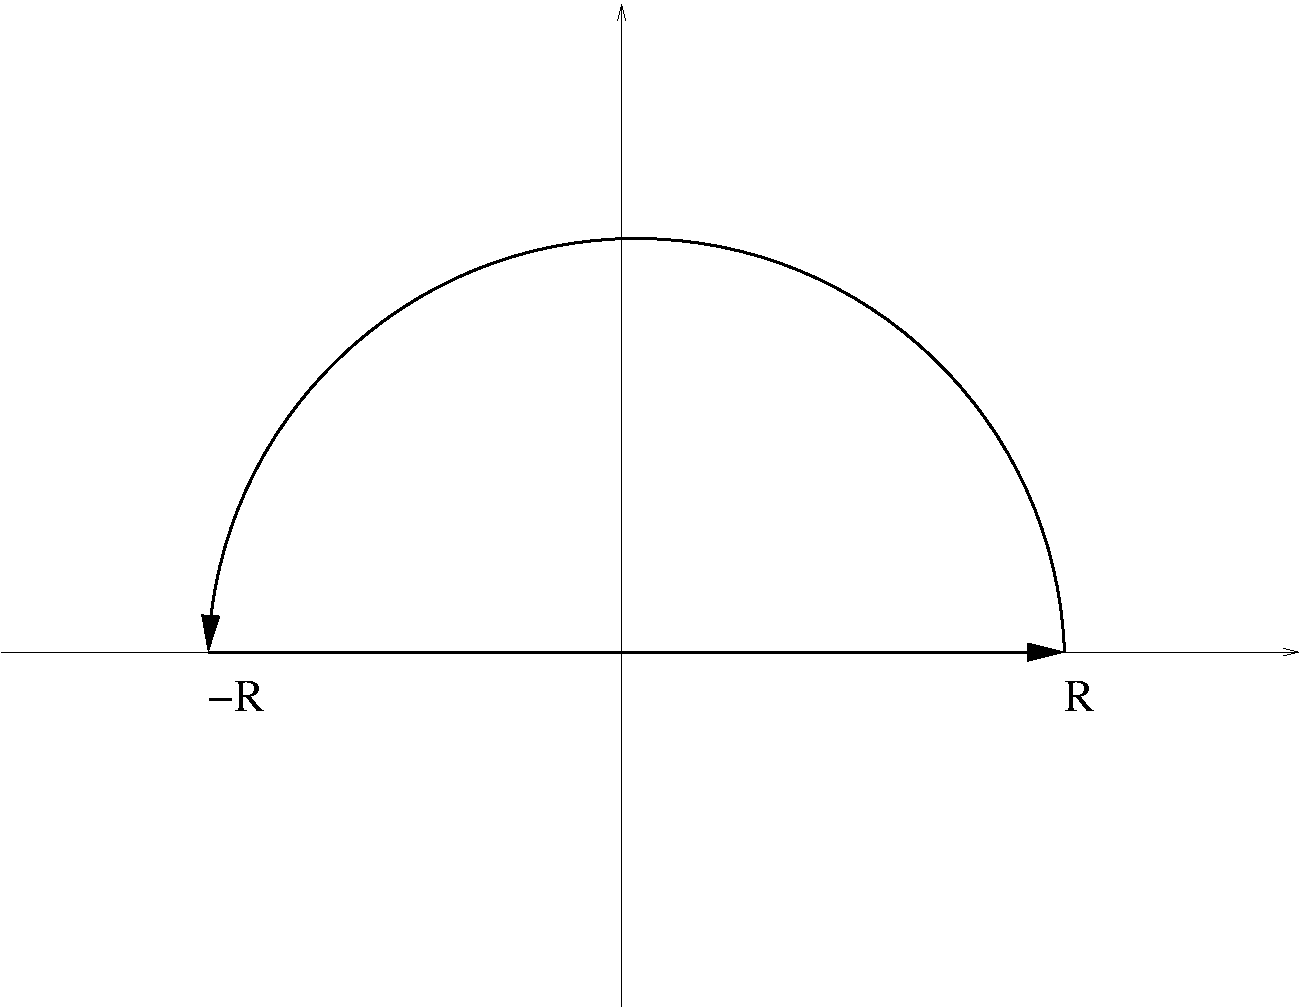
\includegraphics[scale=0.3]{images/contour_ex1.pdf}
\caption{Contour d'intégration}\label{fig:contour_ex1}
\end{figure}
\subsection{Calcul numérique}
Le théorème de Stokes complexe peut être utilisé pour calculer 
numériquement la surface du domaine $\Omega$ entouré par un lacet polygonal $\gamma$. Si 
l'on se donne ce dernier par une liste de sommets $(z_i), \, i=0 \dots N-1$ on peut paramétrer le chemin liant le sommet $i$ au sommet $i+1$ comme:
\[
\gamma_i \colon t \in [0,1] \mapsto z_i + t\left(z_{i+1}-z_i\right)
\]
Sur cette partie du lacet, on formera l'intégrale:
\[
\int_{\gamma_i}\overline{z}dz = \int_{[0,1]}\left(\overline{ z_i}+t \overline{\left(z_{i+1}-z_i\right)}\right)\left(z_{i+1}-z_i\right) dt=
\frac{\overline{z_{i+1}}+\overline{z_i}}{2}\left(z_{i+1}-z_i\right)
\]
et par la formule de Stokes complexe:
\[
\sum_{i=0}^{N-1}\frac{\overline{z_{i+1}}+\overline{z_i}}{2}\left(z_{i+1}-z_i\right) = - \int_{\Omega} dz d\overline{z}
\]
Comme:
\[
\int_{\Omega} dz d\overline{z} = - 2 i \int_{\Omega} dx dy
\]
on en déduit que la surface de $\Omega$ est égale à:
\[
- i \sum_{i=0}^{N-1}\frac{\overline{z_{i+1}}+\overline{z_i}}{4}\left(z_{i+1}-z_i\right)
\]
En développant, on obtient:
\[
- \frac{i}{4} \sum_{i=0}^{N-1} \left(\left|z_{i+1}\right|^2 - \left|z_i \right|^2 + 2 i \Im \left(z_{i+1}\overline{z_i} \right)
\right)
\]
On peut vérifier sans difficultés que les termes en module carré se simplifient deux à deux dans la somme (se rappeler que $z_N = z_0$). La surface est donc en final:
\[
\frac{1}{2} \sum_{i=0}^{N-1} \Im \left(z_{i+1}\overline{z_i} \right)
\]
Enfin, on remarque que pour tout couple $(z_1=x_1+iy_1, z_2=x_2+iy_2)$ le produit $z_2 \overline{z_1}$ a pour partie réelle le produit scalaire des vecteurs $(x_1,y_1)$ et $(x_2,y_2)$ et pour partie réelle leur déterminant. Ceci donne une interprétation géométrique à la formule de sommation précédente, le déterminant de deux vecteurs orientés en sens direct s'identifiant à la surface du parallélogramme qu'ils définissent. Le code python ci-dessous implémente le calcul de surface tel qu'il vient d'être énoncé. 
\begin{verbatim}
# -*- coding: utf8 -*-
import math


# classe point
class Point:
    def __init__(self,x=0.0,y=0.0):
        self.x=x
        self.y=y
# classe lacet
class Lacet:
    # constructeur. La liste de points est initialement vide
    def __init__(self):
        self.point_list=[]
    # ajoute un point à la liste définissant le lacet
    # p : point
    def add(self,p):
        self.point_list.append(p)
    # calcule la surface entourée par le lacet
    # return: réel
    def surface(self):
        surf = 0.0
        n = len(self.point_list)-1
        for i in range(n):
            surf = surf-self.point_list[i+1].x*self.point_list[i].y\
             + self.point_list[i+1].y * self.point_list[i].x
        	surf = surf - self.point_list[0].x*self.point_list[n].y\
        	 + self.point_list[0].y*self.point_list[n].x
        return 0.5 * surf
# test
gamma=Lacet()
gamma.add(Point(1.0,0.0))
gamma.add(Point(0.0,1.0))
gamma.add(Point(-1.0,0.0))
gamma.add(Point(0.0,-1.0))

print(gamma.surface())

gamma=Lacet()
gamma.add(Point(1.0,1.0))
gamma.add(Point(-1.0,1.0))
gamma.add(Point(-1.0,-1.0))
gamma.add(Point(1.0,-1.0))

print(gamma.surface())
\end{verbatim}
A titre d'exercice, améliorer le code pour inclure des lacets définis par des segments de droites et des arcs de cercle. 
\newpage
\leftline{\textbf{Un peu d'histoire \dots}}
\vskip 12pt
\begin{tabular}{ll}
\multicolumn{2}{l}{\textbf{Augustin Louis Cauchy}} \\[10pt]
\begin{minipage}{0.2\linewidth}
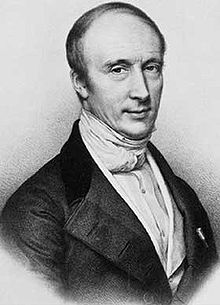
\includegraphics[scale=0.4]{images/Cauchy.jpg}
\end{minipage}
&
\begin{minipage}{0.65\linewidth}
Né le  né à Paris le 21 août 1789 et mort à Sceaux (Hauts-de-Seine) le 23 mai 1857. C'est un des mathématiciens les plus productifs connus (800 publications à son actif). Ses travaux ont concerné la plupart des domaines des mathématiques de son époque: analyse, algèbre, géométrie, probabilités. On lui doit le critère qui porte son nom pour les suites et est à l'origine de la théorie de l'intégration complexe. 
\end{minipage}\\
\multicolumn{2}{l}{\textbf{Edouard Goursat}} \\[10pt]
\begin{minipage}{0.2\linewidth}
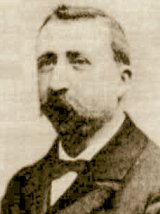
\includegraphics[scale=0.4]{images/Goursat.jpg}
\end{minipage}
&
\begin{minipage}{0.65\linewidth}
 Né le 21 mai 1858 à Lanzac (Lot) et mort le 25 novembre 1936 à Paris. Il travailla sur les fonctions de la variable complexe et prouva le lemme qui porte son nom. Son cours d'analyse a été longtemps une référence.
\end{minipage}
\end{tabular}